\subsection{Chapter 8 - Potential Energy and Conservation of Energy}

\subsubsection{Overview}\label{chapter:potentialecons}

In this chapter, we continue to develop the concept of energy in order to introduce a different formulation for Classical Physics that does not use forces. Although we can describe many phenomena using energy instead of forces, this method is completely equivalent to using Newton's Three Laws. As such, this method can be derived from Newton's formulation, as we will see. Because energy is a scalar quantity, for many problems, it leads to models that are much easier to develop mathematically than if one had used forces. The chapter will conclude with a presentation of the more modern approach, using ``Lagrangian Mechanics'', that is currently preferred in physics and forms the basis for extending our description of physics to the microscopic world (e.g. quantum mechanics).

\begin{framed}
\textbf{Learning Objectives}\\
\begin{itemize}
\item Understand the difference between conservative and non-conservative forces.
\item Understand how to define potential energy for a conservative force.
\item Understand how to use potential energy to calculate work.
\item Understand the definition of mechanical energy.
\item Understand how to use conservation of mechanical energy.
\item Understand how to apply the Lagrangian formulation in a simple case.
\end{itemize}
\end{framed}

\begin{framed}
\textbf{Think About It}\\
Three roller coaster carts start at position $x=0$,  where they are all at the same height (Figure~\ref{fig:potentialecons:rollercoaster}). All of the carts start with the same velocity. At $x_1$, which roller coaster cart will be moving the fastest?

All of the roller coasters end at ground level, at $x_2$. Which roller coaster cart will be moving the fastest at $x_2$? Will all of them make it to $x_2$? Who will get there first?  Assume that the roller coaster track is frictionless.

\begin{figure}[!htbp]
\centering
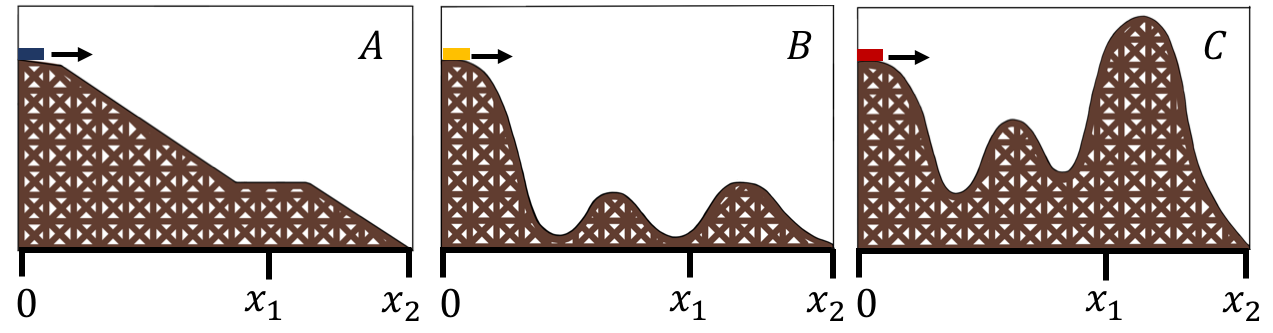
\includegraphics[width=0.9\linewidth]{files/rollercoaster-b808f7c2c4d1e7bad096bad327060c99.png}
\caption[]{Three roller coasters that start at the same height and end at the same height.}
\label{fig:potentialecons:rollercoaster}
\end{figure}

\begin{framed}
\textbf{Answer}\\
All of the carts start at the same height and with the same speed, so they all start with the same mechanical energy. At $x_1$, Cart B is moving the fastest. This is because Cart B is at the lowest height, so more of its gravitational potential energy has been converted into kinetic energy. At $x_2$, Cart A and Cart B will be moving at the same speed because they are at the same height. Cart C will only make it to $x_2$ if it is going fast enough at $x=0$, since it needs to clear bump that is higher than the height it started at. Cart B will be moving the fastest at $x_2$ because throughout the duration of the ride, it is at a lower height on average than Cart A, so its gravitational potential energy is converted to kinetic energy sooner and it gets to the end in less time.
\end{framed}
\end{framed}

\subsubsection{Conservative forces}\label{sec:potentialecons:conservative}

In Section~\ref{chap:workenergy}, we introduced the concept of work, $W$, done by a force, $\vec F(\vec r)$, acting on an object as it moves along a path from position $A$ to position $B$:
\begin{equation}
\label{eq:potentialecons:workdef}
W = \int_A^B \vec F(\vec r) \cdot d\vec l
\end{equation}
where $\vec F(\vec r)$ is a force vector that, in general, is different at different positions in space ($\vec r$). We can also say that $\vec F$ depends on position by writing $\vec F(\vec r)=\vec F(x,y,z)$, since the position vector, $\vec r$, is simply the vector $\vec r = x\hat x + y \hat y+ z\hat z$. That is, $\vec F(\vec r)$ is just a short hand notation for $\vec F(x,y,z)$, and $d\vec l$ is a (very) small segment along the particular path over which one calculates the work.

The above integral is, in general, difficult to evaluate, as it depends on the specific path over which the object moved. In Example~7.2 of Section~\ref{chap:workenergy}, we calculated the work done by friction on a crate that was slid across the floor along two different paths and indeed found that the work depended on the path that was taken. In Example~7.3 of the same chapter, we saw that the work done by the force of gravity when moving a box along two different paths did not depend on the path chosen\footnote{At least for those two paths that we tried in the example.}.

We call ``conservative forces'' those forces for which the work done only depends on the initial and final positions and not on the path taken between those two positions. ``Non-conservative'' forces are those for which the work done does depend on the path taken. The force of gravity is an example of a conservative force, whereas friction is an example of a non-conservative force.

This means that the work done by a conservative force on a ``closed path'' is zero; that is, \textbf{the work done by a conservative force on an object is zero if the object moves along a path that brings it back to its starting position.}
Indeed, since the work done by a conservative force only depends on the location of the initial and final positions, and not the path taken between them, the work has to be zero if the object ends in the same place as where it started (a possible path is for the object to not move at all).

Consider the work done by gravity in raising (displacement $\vec d_1$) and lowering (displacement $\vec d_2= -\vec d_1$) an object back to its starting position along a vertical path, as depicted in Figure~\ref{fig:potentialecons:gravityvertical}.

\begin{figure}[!htbp]
\centering
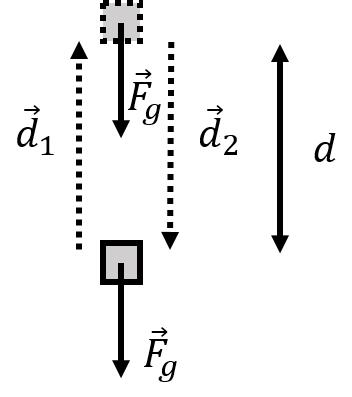
\includegraphics[width=0.2\linewidth]{files/gravityvertical-f825ebbf44bae636c197ad7b8f77b4e6.png}
\caption[]{An object that has moved up and back down.}
\label{fig:potentialecons:gravityvertical}
\end{figure}

The total work done by gravity on this particular closed path is easily shown to be zero, as the work can be broken up into the negative work done as the object moves up (displacement vector $\vec d_1$) and the positive work done as the object moves down (displacement vector $\vec d_2$):
\begin{equation}
W^{tot} = \vec F_g \cdot \vec d_1 + \vec F_g \cdot \vec d_2 = -mgd + mgd = 0
\end{equation}
In order to write the path integral of the force over a closed path, we introduce a new notation to indicate that the starting and ending position are the same:
\begin{equation}
\int_A^A \vec F(\vec r) \cdot d\vec l = \oint \vec F(\vec r) \cdot d\vec l
\end{equation}
The condition for a force to be conservative is thus:
\begin{equation}
\boxed{\oint \vec F(\vec r) \cdot d\vec l = 0}
\end{equation}
since this means that the work done over a closed path is zero. The condition for this integral to be zero can be found by Stokes' Theorem:

\begin{equation}
\oint \vec F(\vec r) \cdot d\vec l = \int_S \left[\left(\frac{\partial F_z}{\partial y}-\frac{\partial F_y}{\partial z}\right)\hat x+ \left(\frac{\partial F_x}{\partial z}-\frac{\partial F_z}{\partial x}\right)\hat y + \left(\frac{\partial F_y}{\partial x}-\frac{\partial F_x}{\partial y}\right)\hat z \right]\cdot d\vec A
\end{equation}
where the integral on the right is called a ``surface integral'' over the surface, $S$, enclosed by the closed path over which the work is being calculated. Don't worry, it is way beyond the scope of this text to understand this integral or Stokes' Theorem in detail! It is however useful in that it gives us the following conditions on the components of a force for that force to be conservative (by requiring the terms in parentheses to be zero):
\begin{equation}
\label{eq:potentialecons:conservative}
\frac{\partial F_z}{\partial y}-\frac{\partial F_y}{\partial z} &= 0 \nonumber\\
\frac{\partial F_x}{\partial z}-\frac{\partial F_z}{\partial x} &= 0\nonumber\\
\frac{\partial F_y}{\partial x}-\frac{\partial F_x}{\partial y} &= 0
\end{equation}
In general:

\begin{enumerate}
\item A force can be conservative if it only depends on position in space, and not speed, time, or any other quantity.
\item A force is conservative if it is constant in magnitude and direction.
\end{enumerate}

\begin{framed}
\textbf{Checkpoint}\\
You push a crate from point $A$ to point $B$ along a horizontal surface. Is the force you exert a conservative force?

\begin{figure}[!htbp]
\centering
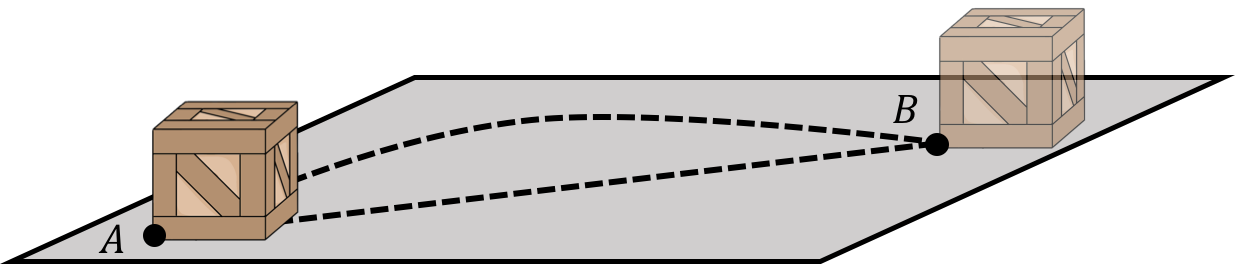
\includegraphics[width=0.7\linewidth]{files/crateab-3d642d5d5d5261439832e71d66ccc56a.png}
\caption[]{You push a crate from A to B along any path.}
\label{fig:potentialecons:cratepath}
\end{figure}

\begin{enumerate}
\item Yes
\item No
\item Not enough information
\end{enumerate}

\begin{framed}
\textbf{Answer}\\
\begin{enumerate}[resume]
\item
\end{enumerate}
\end{framed}
\end{framed}

\begin{framed}
\textbf{Example 8.1}\\
Is the force of gravity on an object of mass $m$, near the surface of the Earth, given by:
\begin{equation}
\vec F(x,y,z) =0\hat x + 0\hat y -mg \hat z
\end{equation}
conservative? Note that we have defined the $z$ axis to be vertical and positive upwards.\}

\begin{framed}
\textbf{Solutions}\\
The force is expected to be conservative since it is constant in magnitude and direction. We can verify this using the conditions in (\ref{eq:potentialecons:conservative}):
\begin{equation}
\frac{\partial F_z}{\partial y}-\frac{\partial F_y}{\partial z} &= \frac{\partial }{\partial y}(-mg) - 0 &= 0\\
\frac{\partial F_x}{\partial z}-\frac{\partial F_z}{\partial x} &= 0 - \frac{\partial }{\partial x}(-mg) &= 0\\
\frac{\partial F_y}{\partial x}-\frac{\partial F_x}{\partial y} &= 0 - 0 &=0
\end{equation}
and the force is indeed conservative since all three conditions are zero.
\end{framed}
\end{framed}

\begin{framed}
\textbf{Example 8.2}\\
Is the following force conservative?
\begin{equation}
\vec F(x,y,z) = \frac{-k}{r^3}\vec r = \frac{-kx}{(x^2+y^2+z^2)^\frac{3}{2}}\hat x + \frac{-ky}{(x^2+y^2+z^2)^\frac{3}{2}}\hat y + \frac{-kz}{(x^2+y^2+z^2)^\frac{3}{2}}\hat z
\end{equation}
\begin{framed}
\textbf{Solution}\\
Since the force only depends on position, it \textit{could} be conservative, so we must check using the conditions from (\ref{eq:potentialecons:conservative}):
\begin{equation}
\frac{\partial F_z}{\partial y}-\frac{\partial F_y}{\partial z} &= \frac{\partial }{\partial y}\left(\frac{-kz}{(x^2+y^2+z^2)^\frac{3}{2}}\right)-\frac{\partial }{\partial z}\left( \frac{-ky}{(x^2+y^2+z^2)^\frac{3}{2}}\right)\\
&=\frac{3kz(2y)}{2(x^2+y^2+z^2)^\frac{5}{2}}-\frac{3ky(2z)}{2(x^2+y^2+z^2)^\frac{5}{2}} = 0\\
\frac{\partial F_x}{\partial z}-\frac{\partial F_z}{\partial x} &= \frac{\partial }{\partial z}\left(\frac{-kx}{(x^2+y^2+z^2)^\frac{3}{2}}\right)-\frac{\partial }{\partial x}\left( \frac{-kz}{(x^2+y^2+z^2)^\frac{3}{2}}\right)\\
&=\frac{3kx(2z)}{2(x^2+y^2+z^2)^\frac{5}{2}}-\frac{3kz(2x)}{2(x^2+y^2+z^2)^\frac{5}{2}} = 0\\
\frac{\partial F_y}{\partial x}-\frac{\partial F_x}{\partial y} &= \frac{\partial }{\partial x}\left(\frac{-ky}{(x^2+y^2+z^2)^\frac{3}{2}}\right)-\frac{\partial }{\partial y}\left( \frac{-kx}{(x^2+y^2+z^2)^\frac{3}{2}}\right)\\
&=\frac{3ky(2x)}{2(x^2+y^2+z^2)^\frac{5}{2}}-\frac{3kx(2y)}{2(x^2+y^2+z^2)^\frac{5}{2}} = 0
\end{equation}
where we used the Chain Rule to take the derivatives. Since all of the conditions are zero, the force is conservative. As we will see, the force represented here is similar mathematically to both the force that Newton introduced in his Universal Theory of Gravity, and the force introduced by Coulomb as the electric force, which are both conservative.
\end{framed}
\end{framed}

\subsubsection{Potential energy}

In this section, we introduce the concept of ``potential energy''. Potential energy is a scalar function of position that can be defined for any conservative force in a way to make it easy to calculate the work done by that force over any path. Since the work done by a conservative force in going from position $A$ to position $B$ does not depend on the particular path taken, but only on the end points, we can write the work done by a conservative force in terms of a ``potential energy function'', $U(\vec r)$, that can be evaluated at the end points:
\begin{equation}
\boxed{-W = - \int_A^B \vec F(\vec r) \cdot d\vec l = U(\vec r_B) - U(\vec r_A) = \Delta U}
\end{equation}
where we have have chosen to define the function $U(\vec r)$ so that it relates to the \textbf{negative} of the work done for reasons that will be apparent in the next section. Figure~\ref{fig:potentialecons:potentialpath} shows an example of an arbitrary path between two points $A$ and $B$ in two dimensions for which one could calculate the work done by a conservative force using a potential energy function.

\begin{figure}[!htbp]
\centering
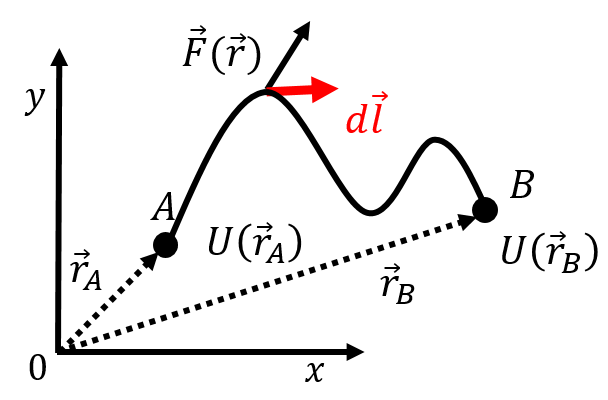
\includegraphics[width=0.4\linewidth]{files/potentialpath-a6e90e6b49e93ae93bfdae02b8783087.png}
\caption[]{Illustration of calculating the work done by a conservative function along an arbitrary path by taking the difference in potential energy evaluated at the two endpoints, $-W=U(\vec r_B) - U(\vec r_A)$.}
\label{fig:potentialecons:potentialpath}
\end{figure}

Once we know the function for the potential energy, $U(\vec r)$, we can calculate the work done by the associated force along any path. In order to determine the function, $U(\vec r)$, we can calculate the work that is done along a path over which the integral for work is easy (usually, a straight line).

For example, near the surface of the Earth, the force of gravity on an object of mass, $m$, is given by:
\begin{equation}
\vec F_g = -mg \hat z
\end{equation}
where we have defined the $z$ axis to be vertical and positive upwards. We already showed in Example~8.1 that this force is conservative and that we can thus define a potential energy function. To do so, we can calculate the work done by the force of gravity over a straight vertical path, from position $A$ to position $B$, as shown in Figure~\ref{fig:potentialecons:gravitydl}.

\begin{figure}[!htbp]
\centering
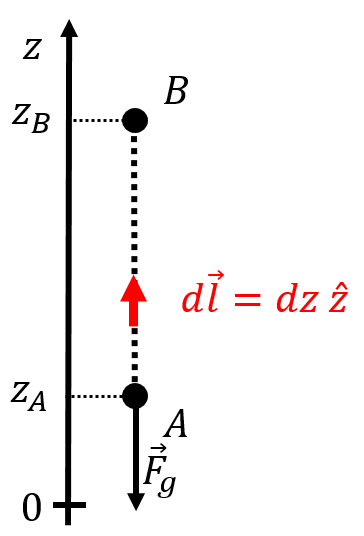
\includegraphics[width=0.2\linewidth]{files/gravitydl-5d65187a9c22e9b4b1279569b7a8958e.png}
\caption[]{A vertical path for calculating the work done by gravity.}
\label{fig:potentialecons:gravitydl}
\end{figure}

The work done by gravity from position $A$ to position $B$ is:
\begin{equation}
W &= \int_A^B \vec F(\vec r) \cdot d\vec l\\
&= \int_{z_A}^{z_B} ( -mg \hat z) \cdot (dz \hat z) \\
&= -mg \int_{z_A}^{z_B} dz\\
&= -mg(z_B-z_A)
\end{equation}
By inspection, we can now identify the functional form for the potential energy function, $U(\vec r)$. We require that:
\begin{equation}
-W &= U(\vec r_B) - U(\vec r_A) = U(z_B) - U(z_A)
\end{equation}
where we replaced the position vector, $\vec r$, with the $z$ coordinate, since this is a one dimensional situation. Therefore:
\begin{equation}
-W=mg(z_B-z_A)&= U(z_B) - U(z_A)\\
\therefore U(z) &= mgz + C
\end{equation}
and we have found that, for the force of gravity near the surface of the Earth, one can define a potential energy function (by inspection), $U(z) = mgz +C$.

It is important to note that, since it is only the \textbf{difference} in potential energy that matters when calculating the work done, the potential energy function can have an arbitrary constant, $C$, added to it. Thus, \textbf{the value of the potential energy function is meaningless, and only differences in potential energy are meaningful and related to the work done on an object}. In other words, it does not matter where the potential energy is equal to zero, and by choosing $C$, we can therefore choose a convenient location where the potential energy is zero.

\begin{framed}
\textbf{Checkpoint}\\
When we found the work done by gravity, we defined positive $z$ to be upwards. If we instead chose positive $z$ to be downwards, how would the potential energy function be defined?

\begin{enumerate}
\item The potential energy function would be the same, $U(z)=mgz+C$.
\item The potential energy function would be the same but negative, $U(z)= -mgz+C$
\end{enumerate}

\begin{framed}
\textbf{Answer}\\
\begin{enumerate}[resume]
\item
\end{enumerate}
\end{framed}
\end{framed}

\begin{framed}
\textbf{Checkpoint}\\
Can an object have a negative potential energy?

\begin{enumerate}
\item Yes
\item No
\end{enumerate}

\begin{framed}
\textbf{Answer}\\
\begin{enumerate}
\item
\end{enumerate}
\end{framed}
\end{framed}

\begin{framed}
\textbf{Example 8.3}\\
Calculate the work done \textbf{by the force of gravity} when a box of mass, $m$, is moved from the ground up onto a table that is a distance $L$ away horizontally and $H$ vertically, as illustrated in Figure~\ref{fig:potentialecons:table}. How much work must be done by a person moving the box?

\begin{figure}[!htbp]
\centering
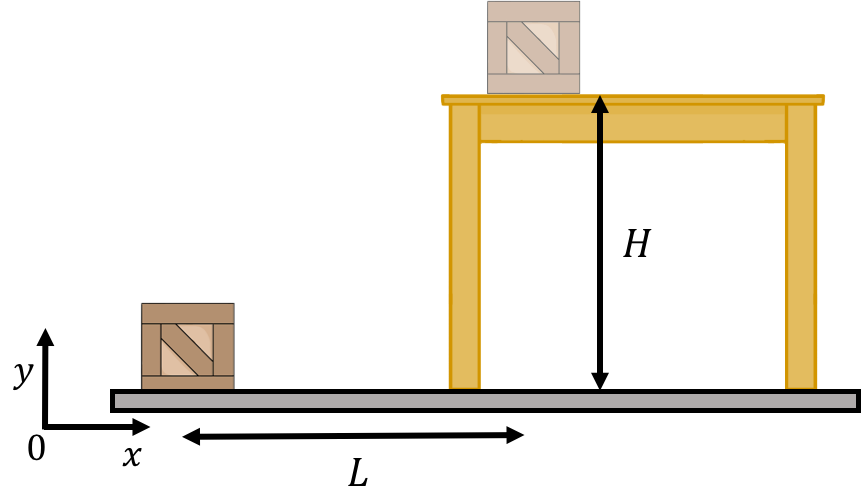
\includegraphics[width=0.5\linewidth]{files/table-86ad09cede94af5d2444e9e90a6ce65a.png}
\caption[]{A box moved from the ground up onto a table.}
\label{fig:potentialecons:table}
\end{figure}

\begin{framed}
\textbf{Solution}\\
Since the force of gravity is conservative, we can use the potential energy function given by:
\begin{equation}
U(z)=mgz+C
\end{equation}
to calculate the work done by the force of gravity when the box is moved. The work done by gravity will only depend on the change in height, $H$, as the potential energy function only depends on the $z$ coordinate of an object.  We can choose the origin of our coordinate system to be the ground and choose the constant $C=0$, so that the potential energy function at the starting position of the box is:
\begin{equation}
U(z_A=0) = mg(0)= 0
\end{equation}
The potential energy function when the box is on the table, with $z=H$, is given by:
\begin{equation}
U(z_B=H) = mgH
\end{equation}
The change in potential energy, $\Delta U = U(z_B) - U(z_A)$ is equal to the negative of the work done by gravity. The work done by gravity, $W_g$, is thus:
\begin{equation}
-W_g &=  U(z_B) - U(z_A) = mgH - 0\\
\therefore W_g &= -mgH
\end{equation}
which is the same as what we found in Example~7.3 of Section~\ref{chap:workenergy}. The work done by gravity is negative, as we found previously. This makes sense because gravity has a component opposite to the direction of motion.

The work done by a person, $W_p$, to move the box can easily be found by considering the net work done on the box. While the box is moving, only the person and gravity are exerting forces on the box, so those are the only two forces performing work. Since the box starts and ends at rest, the net work done on the box must be zero (no change in kinetic energy, recall the Work-Energy Theorem):
\begin{equation}
W^{net} = 0 &= W_g + W_p\\
\therefore W_p &= -W_g = mgH
\end{equation}
\textbf{Discussion:} We find that the person had to do positive work, which makes sense, since they had to exert a force with a component in the direction of motion (upwards). It is also interesting to note that it does not matter if the person exerted a constant force or whether they varied the force that they exerted on the box as they moved it: the amount of work done by the person is fixed to be the negative of the work done by gravity.
\end{framed}
\end{framed}

\begin{framed}
\textbf{Example 8.4}\\
The force exerted by a spring that is extended or compressed by a distance, $x$, is given by Hooke's Law:
\begin{equation}
\vec F(x) = -k x\hat x
\end{equation}
where the $x$ axis is defined to be co-linear with the spring and the origin is located at the rest position of the spring. Show that the force exerted by the spring onto an object is conservative and determine the corresponding potential energy function.

\begin{framed}
\textbf{Solution}\\
Since the force depends on position, it could be conservative, which we can check with the conditions from (\ref{eq:potentialecons:conservative}):
\begin{equation}
\frac{\partial F_z}{\partial y}-\frac{\partial F_y}{\partial z} &= 0 - 0 &= 0\\
\frac{\partial F_x}{\partial z}-\frac{\partial F_z}{\partial x} &= \frac{\partial }{\partial z}(-kx)) - 0&= 0\\
\frac{\partial F_y}{\partial x}-\frac{\partial F_x}{\partial y} &= 0 - \frac{\partial }{\partial y}(-kx)) &=0
\end{equation}
and the force is indeed conservative. To determine the potential energy function, let us calculate the work done by the spring from position $x_A$ to position $x_B$:
\begin{equation}
W &=\int_A^B \vec F(\vec r) \cdot d\vec l\\
&=\int_{x_A}^{x_B} (-kx\hat x) \cdot dx \hat x\\
&=\int_{x_A}^{x_B} (-kx)dx=\left[-\frac{1}{2}kx^2  \right]_{x_A}^{x_B}\\
&=-\left( \frac{1}{2}kx_B^2-\frac{1}{2}kx_A^2 \right)
\end{equation}
Again, comparing with:
\begin{equation}
-W &= U(\vec r_B) - U(\vec r_A) = U(x_B) - U(x_A)
\end{equation}
We can identify the potential energy for a spring:
\begin{equation}
U(x) = \frac{1}{2}kx^2 + C
\end{equation}
where, in general, the constant $C$ can take any value. If we choose $C=0$, then the potential energy is zero when the spring is at rest, although it is not important what choice is made. Note that in one dimension, the potential energy function is the negative of the anti-derivative of the function that gives the $x$ component of the force.
\end{framed}
\end{framed}

\begin{framed}
\textbf{Checkpoint}\\
A conservative force acts on an object that is initially at rest. No other forces act on the object. Does the object move in a way that increases its potential energy or decreases its potential energy?

\begin{enumerate}
\item Increases.
\item Decreases.
\item It depends on the choice of $C$ for the corresponding potential energy.
\end{enumerate}

\begin{framed}
\textbf{Answer}\\
\begin{enumerate}[resume]
\item
\end{enumerate}
\end{framed}
\end{framed}

\paragraph{Recovering the force from potential energy}\label{sec:potentialecons:forcefromu}

Given a (scalar) potential energy function, $U(\vec r)$, it is possible to determine the (vector) force that is associated with it. Take, for example, the potential energy from a spring (Example~8.4):
\begin{equation}
U(x) = \frac{1}{2}kx^2 + C
\end{equation}
As you recall from Example~8.4, to find this function (in one dimension), we took the $x$ component of the spring force and (effectively) found the negative of its anti-derivative, which we defined as the potential energy function:
\begin{equation}
F(x) &= -kx\\
U(x) &= -\int F(x) dx = \int (kx) dx = \frac{1}{2}kx^2+C\\
\therefore F(x) &= -\frac{d}{dx}U(x)
\end{equation}
Thus, the force can be obtained from the negative of the potential energy function, by taking its derivative with respect to position.

In three dimensions, the situation is similar, although the potential energy function (and the components of the force vector) will generally depend on all three position coordinates, $x$, $y$, and $z$. In three dimensions, the the three components of the force vector are given by taking the gradient of the negative of the potential energy function\footnote{As you may recall from Section~\ref{app:calculus}, the gradient is a vector that points towards the direction of maximal increase in a multi-variate function.}:
\begin{equation}
\vec F(\vec r) &= -\vec\nabla U(\vec r)=-\vec\nabla U(x,y,z)\nonumber\\
\therefore F_x(x,y,z) &= -\frac{\partial }{\partial x}U(x,y,z)\nonumber\\
\therefore F_y(x,y,z) &= -\frac{\partial }{\partial y}U(x,y,z)\nonumber\\
\therefore F_z(x,y,z) &= -\frac{\partial }{\partial z}U(x,y,z)
\end{equation}

\subsubsection{Mechanical energy and conservation of energy}

Recall the Work-Energy Theorem, which relates the net work done on an object to its change in kinetic energy, along a path from point $A$ to point $B$:
\begin{equation}
W^{net}=\Delta K = K_B - K_A
\end{equation}
where $K_A$ is the object's initial kinetic energy and $K_B$ is its final kinetic energy. Generally, the net work done is the sum of the work done by conservative forces, $W^C$, and the work done by non-conservative forces, $W^{NC}$:
\begin{equation}
W^{net}=W^C+W^{NC}
\end{equation}
The work done by conservative forces can be expressed in terms of changes in potential energy functions. For example, suppose that two conservative forces, $\vec F_1$ and $\vec F_2$, are exerted on the object. The work done by those two forces is given by:
\begin{equation}
W_1 &= -\Delta U_1\\
W_2 &= -\Delta U_2
\end{equation}
where $U_1$ and $U_2$ are the changes in potential energy associated with forces $\vec F_1$ and $\vec F_2$, respectively. We can re-arrange the Work-Energy Theorem as follows\footnote{This is why we defined potential energy as negative of the work; it becomes a positive term when we move it to the same side of the equation as the kinetic energy!}:
\begin{equation}
W^{net}=W^C+W^{NC}=-\Delta U_1 - \Delta U_2 +W^{NC} &= \Delta K\\
\therefore W^{NC} = \Delta U_1 + \Delta U_2 + \Delta K
\end{equation}
That is, the work done by non-conservative forces is equal to the sum of the changes in potential and kinetic energies. In general, we can use $\Delta U$ to represent the change in the total potential energy of the object. The total potential energy is the sum of the potential energies associated with each of the conservative forces acting on the object ($\Delta U = \Delta U_1 + \Delta U_2$ above). The above expression can thus be written in a more general form:
\begin{equation}
\boxed{W^{NC}=\Delta U + \Delta K}
\end{equation}
In particular, note that if there are no non-conservative forces doing work on the object:
\begin{equation}
\boxed{\Delta K + \Delta U = 0}\\
-\Delta U = \Delta K \quad\text{if no non-conservative forces}
\end{equation}
That is, the sum of the changes in potential and kinetic energies of the object is always zero. This means that if the potential energy of the object increases, then the kinetic energy of the object must decrease by the same amount.

We can introduce the ``mechanical energy'', $E$, of an object as the sum of the potential and kinetic energies of the object:
\begin{equation}
\boxed{E = U+K}
\end{equation}
If the object started at position $A$, with potential energy $U_A$ and kinetic energy $K_A$, and ended up at position $B$ with potential energy $U_B$ and kinetic energy $K_B$, then we can write the mechanical energy at both positions and its change $\Delta E$, as:
\begin{equation}
E_A &= U_A + K_A\\
E_B &= U_B + K_B\\
\Delta E &= E_B - E_A \\
&= U_B + K_B - U_A - K_A\\
\therefore \Delta E &= \Delta U + \Delta K
\end{equation}
Thus, the change in mechanical energy of the object is equal to the work done by non-conservative forces:
\begin{equation}
W^{NC} = \Delta U + \Delta K = \Delta E
\end{equation}
and if there is no work done by non-conservative forces on the object, then the mechanical energy of the object does not change:
\begin{equation}
\Delta E &= 0\quad\text{if no non-conservative forces}\\
\therefore E &= \text{constant}
\end{equation}
This is what we generally call the ``conservation of mechanical energy''. If there are no non-conservative forces doing work on an object, its mechanical energy is conserved (i.e. constant).

The introduction of mechanical energy gives us a completely different way to think about mechanics. We can now think of an object as having ``energy'' (potential and/or kinetic), and we can think of forces as changing the energy of the object.

\begin{framed}
\textbf{Checkpoint}\\
Is the value of an an object's mechanical energy meaningful, or is it only the difference in mechanical energy that is meaningful?

\begin{enumerate}
\item Yes, the value of the mechanical energy is meaningful. At any given time, an object will have a quantifiable amount of mechanical energy.
\item No, the value is not meaningful because the value of potential energy is arbitrary. Only differences in mechanical energy are meaningful.
\item No, the value is not meaningful because both the potential and kinetic energies are arbitrary. Their values will change depending on where you set the energy to be zero.
\item It depends on which conservative forces act on the object (and therefore what ``kind'' of potential energy the object has).
\end{enumerate}

\begin{framed}
\textbf{Answer}\\
\begin{enumerate}[resume]
\item
\end{enumerate}
\end{framed}
\end{framed}

We can also think of the work done by non-conservative forces as a type of change in energy. For example, the work done by friction can be thought of as a change in thermal energy (feel the burn as you rub your hand vigorously on a table!). If we can model the work done by non-conservative forces as a type of ``other'' energy, $-W^{NC}=\Delta E^{other}$, then we can state that:
\begin{equation}
\Delta E^{other} + \Delta U + \Delta K =0
\end{equation}
which is what we usually refer to as ``conservation of energy''. That is, the total energy in a system, including kinetic, potential and any other form (e.g. thermal, electrical, etc.) is constant unless some external agent is acting on the system.

We can always include that external agent in the system so that the total energy of the system is constant. The largest system that we can have is the Universe itself. Thus, the total energy in the Universe is constant and can only transform from one type into another, but no energy can ever be added or removed from the Universe.

\begin{framed}
\textbf{Olivia's Thoughts}\\
Here's an example that may help you understand the concept of external agents and energy conservation. Say we have a mass that hangs from a spring, so that the mass oscillates up and down like a yo-yo. If we define our system to include the spring, the mass, and gravity, energy will be conserved (the energy is transformed from potential energy to kinetic energy and back again).

Now, what if someone is holding the end of the spring and they start walking so that the whole system accelerates? Energy is not conserved because the system is gaining kinetic energy, seemingly out of nowhere. The system is being acted on by an \textit{external agent} (the person). If we expand our system so that it includes the spring, the mass, gravity, \textit{and the person}, energy is conserved. Instead of the kinetic energy ``coming out of nowhere'', we can see that it is actually coming from the person converting chemical energy in their body in order to move their muscles.

\begin{figure}[!htbp]
\centering
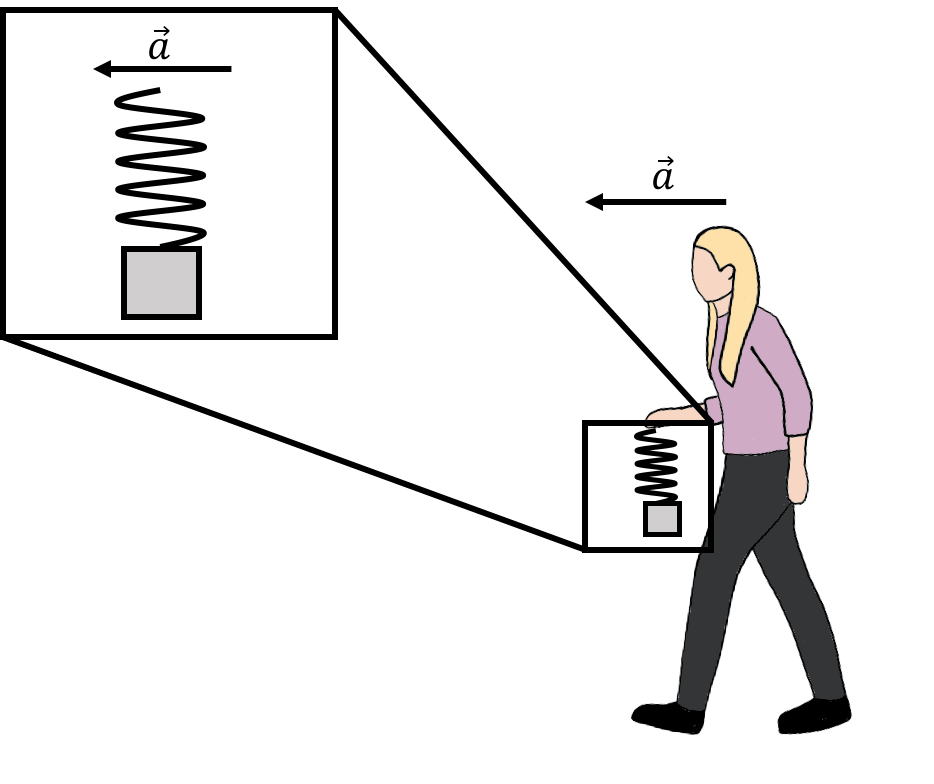
\includegraphics[width=0.4\linewidth]{files/externalagentex-66771caacaa3f48d61e159995851589f.png}
\caption[]{A person accelerates a mass and spring by walking. If the system does not include the person, energy is not conserved. If it does include the person, energy is conserved.}
\label{fig:potentialecons:externalagentx}
\end{figure}

But what if there's an external agent acting on our new system? We can keep ``zooming out'' to include more and more external sources in the definition of our system. If you kept zooming out, eventually you would reach the point where the whole Universe was included in your system. At this point, you can't zoom out any more. This means that, if the Universe is your system, energy must always be conserved because there can't be any external agents acting on the system.
\end{framed}

\begin{framed}
\textbf{Example 8.5}\\
\begin{figure}[!htbp]
\centering
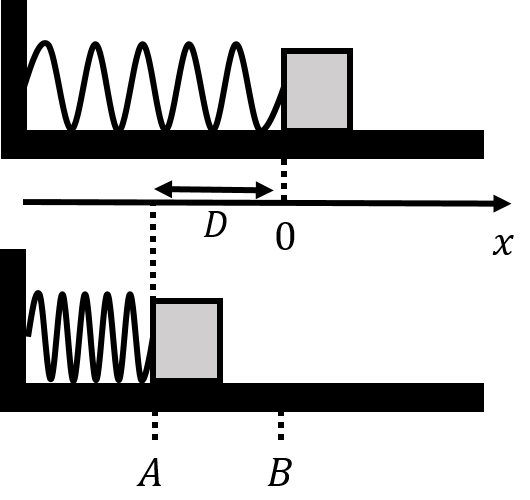
\includegraphics[width=0.4\linewidth]{files/blockspring-5094bde59d2625146e6655fc2e2cf358.png}
\caption[]{A block is launched along a frictionless surface by compressing a spring by a distance $D$. The top panel shows the spring when at rest, and the bottom panel shows the spring compressed by a distance $D$ just before releasing the block.}
\label{fig:potentialecons:blockspring}
\end{figure}

A block of mass $m$ can slide along a horizontal frictionless surface. A horizontal spring, with spring constant, $k$, is attached to a wall on one end, while the other end can move, as shown in Figure~\ref{fig:potentialecons:blockspring}. A coordinate system is defined such that the $x$ axis is horizontal and the free end of the spring is at $x=0$ when the spring is at rest. The block is pushed against the spring so that the spring is compressed by a distance $D$. The block is then released. What speed will the block have when it leaves the spring?

\begin{framed}
\textbf{Solution}\\
This is again the same example that we saw in Section~\ref{chap:ApplyingNewtonsLaws} and Section~\ref{chap:workenergy}. We will show here that it is solved very easily using conservation of energy. The forces acting on the block are:

\begin{enumerate}
\item Weight, which does no work since it is perpendicular to the block's displacement.
\item The normal force, which does no work since it is perpendicular to the block's displacement.
\item The force from the spring, which is conservative and can be modelled with a potential energy $U(x)=\frac{1}{2}kx^2$, where $x$ is the position of the end of the spring.
\end{enumerate}

The block starts at rest at position $A$ ($x= -D$), where the spring is compressed by a distance $D$, and leaves the spring at position $B$ ($x=0$), where the spring is at its rest position.

At position $A$, the kinetic energy of the block is $K_A=0$ since the block is at rest, and the potential energy from the spring force of the block is $U_A=\frac{1}{2}kD^2$. The mechanical energy of the block at position $A$ is thus:
\begin{equation}
K_A&=0\\
U_A&=\frac{1}{2}kD^2\\
\therefore E_A &= U_A + K_A = \frac{1}{2}kD^2
\end{equation}
At position $B$, the spring potential energy of the block is zero (since the spring is at rest), and all of the energy is kinetic:
\begin{equation}
K_B&=\frac{1}{2}mv_B^2\\
U_B&=0\\
\therefore E_B &= U_B+K_B=\frac{1}{2}mv_B^2
\end{equation}
Since there are no non-conservative forces doing work on the block, the mechanical energies at $A$ and $B$ are the same:
\begin{equation}
W^{NC}&=\Delta E=E_B-E_A= 0\\
\therefore E_B&=E_A\\
\frac{1}{2}mv_B^2&= \frac{1}{2}kD^2\\
 v_B &= \sqrt{\frac{kD^2}{m}}
\end{equation}
as we found previously.
\end{framed}
\end{framed}

\begin{framed}
\textbf{Example 8.6}\\
\begin{figure}[!htbp]
\centering
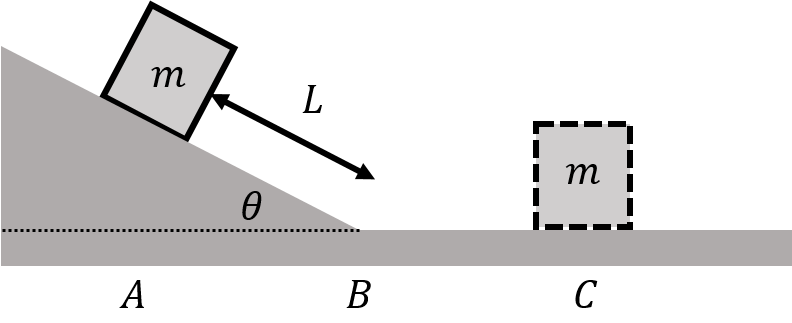
\includegraphics[width=0.5\linewidth]{files/blockI-932a28c0a09a5e6695d86a4eee39dcf0.png}
\caption[]{A block slides down an incline before sliding on a flat surface and stopping.}
\label{fig:potentialecons:blockI}
\end{figure}

A block of mass $m$ is placed at rest on an incline that makes an angle $\theta$ with respect to the horizontal, as shown in Figure~\ref{fig:potentialecons:blockI}. The block is nudged slightly so that the force of static friction is overcome and the block starts to accelerate down the incline. At the bottom of the incline, the block slides on a horizontal surface.
The coefficient of kinetic friction between the block and the incline is $\mu_{k1}$, and the coefficient of kinetic friction between the block and horizontal surface is $\mu_{k2}$. If one assumes that the block started at rest a distance $L$ from the bottom of the incline, how far along the horizontal surface will the block slide before stopping?

\begin{framed}
\textbf{Solution}\\
This is the same problem we solved in this Figure~\ref{fig:applyingnewtonslaws:blockI}. In that case, we solved for the acceleration of the block using Newton's Second Law and then used kinematics to find how far the block went. We can solve this problem in a much easier way using conservation of energy.

It is still a good idea to think about what forces are applied on the object in order to determine if there are non-conservative forces doing work. In this case, the forces on the block are:

\begin{enumerate}
\item The normal force, which does no work, as it is always perpendicular to the motion.
\item Weight, which does work when the height of the object changes, which we can model with a potential energy function.
\item Friction, which is a non-conservative force, whose work we must determine.
\end{enumerate}

Let us divide the motion into two segments: (1) a segment along the incline (positions $A$ to $B$ in Figure~\ref{fig:potentialecons:blockI}), where gravitational potential energy changes, and (2), the horizontal segment from positions $B$ to position $C$ on the figure. We can then apply conservation of energy for each segment.

Starting with the first segment, we can choose the gravitational potential energy to be zero when the block is at the bottom of the incline. The block starts at a height $h=L\sin\theta$ above the  bottom of the incline. The gravitational potential energy for the beginning and end of the first segment are thus:
\begin{equation}
U_A &= mgL\sin\theta\\
U_B &= 0
\end{equation}
Since the block starts at rest, its kinetic energy is zero at position $A$, and if the speed of the box is $v_B$ at position $B$, we can write its kinetic energy at both positions as:
\begin{equation}
K_A &=0\\
K_B &= \frac{1}{2}mv_B^2
\end{equation}
The mechanical energy of the object at positions $A$ and $B$ is thus:
\begin{equation}
E_A &= U_A+K_A = mgL\sin\theta\\
E_B &= U_B+K_B = \frac{1}{2}mv_B^2\\
\Delta E &= E_B - E_A = \frac{1}{2}mv_B^2 - mgL\sin\theta
\end{equation}
Finally, since we have a non-conservative force, the force of kinetic friction, acting on the first segment, we need to calculate the work done by that force. We found in Example~6.2 that the force of friction had magnitude $f_k=\mu_{k1}N=\mu_{k1}mg\cos\theta$. Since the force of friction is anti-parallel to the displacement vector, which points down the incline and has length $L$, the work done by friction is:
\begin{equation}
W^{NC}=W_f = -f_kL=-\mu_{k1}mg\cos\theta L
\end{equation}
Applying conservation of energy along the first segment, we have:
\begin{equation}
W^{NC} &= \Delta E\\
-\mu_{k1}mg\cos\theta L &= \frac{1}{2}mv_B^2 - mgL\sin\theta\\
\therefore \frac{1}{2}mv_B^2 &= mgL\sin\theta-\mu_{k1}mg\cos\theta L
\end{equation}
Note that the above equation, in words, could be read as, ``the change in kinetic energy ($\frac{1}{2}mv_B^2$) is equal to the negative change in potential energy ($mgL\sin\theta$) minus the work done by friction ($\mu_{k1}mg\cos\theta L$)''. In other words, the block had potential energy, which was converted into kinetic energy and heat (the work done by friction can be thought of as thermal energy).

We now proceed in an analogous way for the second segment, from position $B$ to position $C$. The only force that can do work along this segment (of length $x$) is the force of kinetic friction, since both the weight and normal force are perpendicular to the displacement. There are no conservative forces doing work, so there is no change in potential energy. The initial kinetic energy is $K_B$ (from above), and the final kinetic energy, $K_C$, is zero. The change in mechanical energy is thus:
\begin{equation}
\Delta E &= E_C - E_B = K_C - K_B = -K_B\\
&=-\frac{1}{2}mv_B^2\\
&=- mgL\sin\theta+\mu_{k1}mg\cos\theta L
\end{equation}
where, in the last line, we used the result from the first segment. The work done by the force of friction along the horizontal segment of (undetermined) length $x$ is:
\begin{equation}
W^{NC}=W_f = -f_kx = -\mu_{k2} N x=-\mu_{k2} mg x
\end{equation}
Finally, we can find $x$ by setting the work done by non-conservative forces equal to the change in mechanical energy:
\begin{equation}
W^{NC} &= \Delta E\\
-\mu_{k2} mg x &=- mgL\sin\theta+\mu_{k1}mg\cos\theta L \\
\therefore x&= L\frac{1}{\mu_{k2}}\left(\sin\theta - \mu_{k1}\cos\theta\right)
\end{equation}
which is the same result that we obtained in Example~6.2.

\textbf{Discussion:} By using conservation of energy, we were able to model the motion of the block down the incline in a way that was much easier than what was done in Example~6.2. Furthermore, although we modelled friction as a non-conservative force doing work, we gained some insight into the idea that this could be thought of as an energy loss. In terms of energy, we would say that the block initially had gravitational potential energy, which was then converted into kinetic energy as well as thermal energy (in the heat generated by friction).
\end{framed}
\end{framed}

\subsubsection{Energy diagrams and equilibria}\label{sec:potentialecons:ediagrams}

We can write the mechanical energy of an object as:
\begin{equation}
E = K + U
\end{equation}
which will be a constant if there are no non-conservative forces doing work on the object. This means that if the potential energy of the object increases, then its kinetic energy must decrease by the same amount, and vice-versa.

Consider a block that can slide on a frictionless horizontal surface and that is attached to a spring, as is shown in Figure~\ref{fig:potentialecons:springE} (left side), where $x=0$ is chosen as the position corresponding to the rest length of the spring. If you push on the block so as to compress the spring by a distance $D$ and then release it, the block will initially accelerate because of the spring force in the positive $x$ direction until the block reaches the rest position of the spring ($x=0$ on the diagram). When it passes that point, the spring will exert a force in the opposite direction. The block will continue in the same direction and decelerate until it stops and turns around. It will then accelerate again towards the rest position of the spring, and then decelerate once the spring starts being compressed again, until the block stops and the motion repeats. We say that the block ``oscillates'' back and forth about the rest position of the spring.

We can describe the motion of the block in terms of its total mechanical energy, $E$. Its potential energy is given by:
\begin{equation}
U(x)=\frac{1}{2}kx^2
\end{equation}
On the right of Figure~\ref{fig:potentialecons:springE} is an ``Energy Diagram'' for the block, which allows us to examine how the total energy, $E$, of the block is divided between kinetic and potential energy depending on the position of the block. The vertical axis corresponds to energy and the horizontal axis corresponds to the position of the block.

The total mechanical energy, $E=25 {\rm J}$, is shown by the horizontal red line. Also illustrated are the potential energy function ($U(x)$ in blue), and the kinetic energy, ($K=E -U(x)$, in dotted black).

\begin{figure}[!htbp]
\centering
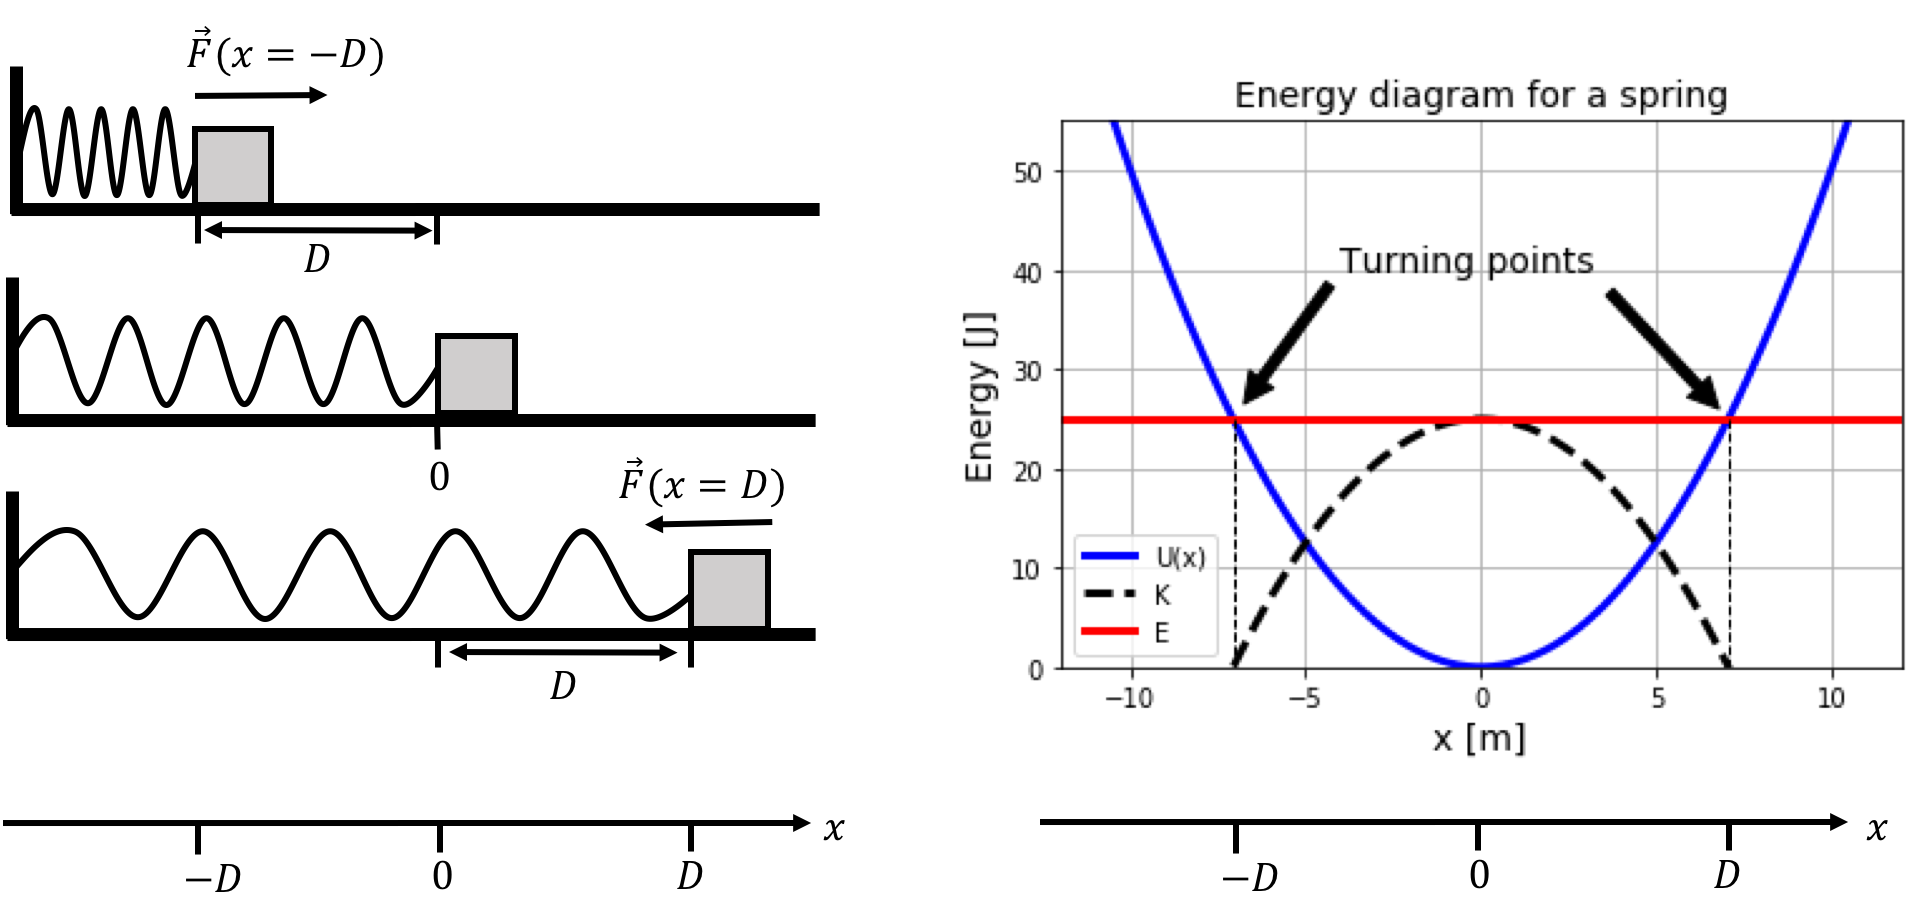
\includegraphics[width=1\linewidth]{files/springE-eaf9354703557107d14f7d6c630c1335.png}
\caption[]{Left: The block oscillates about the rest position of the spring, between $x= -D$ and $x=D$. Right: The energy diagram for the block. This diagram is for a spring with spring constant $k=1 {\rm N/m}$.}
\label{fig:potentialecons:springE}
\end{figure}

The energy diagram allows us to describe the motion of the object attached to the spring in terms of energy. A few things to note:

\begin{enumerate}
\item At $x=\pm D$, the potential energy is equal to $E$, so the kinetic energy is zero. The block is thus instantaneously at rest at those positions.
\item At $x=0$, the potential energy is zero, and the kinetic energy is maximal. This corresponds to where the block has the highest speed.
\item The kinetic energy of the block can never be negative\footnote{Remember, the kinetic energy is given by $K=\frac{1}{2}mv^2$. Since neither mass nor the value of $v^2$ can be negative, the kinetic energy of an object can never be negative.}, thus, the block cannot be located outside the range $[ -D,+D]$, and we would say that the motion of the block is ``bound''. The points between which the motion is bound are called ``turning points''.
\end{enumerate}

An analysis of the energy diagram tells us that the block is bound between the two turning points, which themselves are equidistant from the origin. When we initially compress the spring, we are ``giving'' the block ``spring potential energy''. As the block starts to move, the potential energy of the block is converted into kinetic energy as it accelerates and then back into potential energy as it decelerates.

\begin{framed}
\textbf{Checkpoint}\\
Calculate the positions of the turning points for the situation shown in Figure~\ref{fig:potentialecons:springE}. The total energy is $25 {\rm J}$ and the spring constant is $k=1 {\rm N/m}$.

\begin{framed}
\textbf{Answer}\\
$7.1 {\rm m}$
\end{framed}
\end{framed}

By looking at only the potential energy function, without knowing that it is related to a spring, we can come to the same conclusions; namely that the motion is bound as long as the total mechanical energy is not infinite. We call the point $x=0$ a ``stable equilibrium'', because it is a local minimum of the potential energy function. If the object is displaced from the equilibrium point, it will want to move back towards that point. This can also be understood in terms of the force associated with the potential energy function:
\begin{equation}
F = -\frac{d}{dx}U(x)
\end{equation}
The local minimum occurs where the derivative of the potential function is equal to zero. Thus, the \textbf{equilibrium point is given by the condition that the force associated with the potential is zero} ($x=0$ in the case of the potential energy from a spring). The equilibrium is a stable equilibrium because the force associated with the potential energy function ($F(x)= -kx$ for the spring) points towards the equilibrium point.

The potential energy function for an object with total mechanical energy, $E$, can be thought of as a little ``roller coaster'', on which you place a marble and watch it ``roll down'' the potential energy function. You can think of placing a marble where $U(x)=E$ and releasing it. The marble would then roll down the potential energy function, just as an actual marble would roll down a real slope, mimicking the motion of the object along the $x$ axis. This is illustrated in Figure~\ref{fig:potentialecons:potential} which shows an arbitrary potential energy function and a marble being placed at a location where the potential energy is equal to $E$.

\begin{figure}[!htbp]
\centering
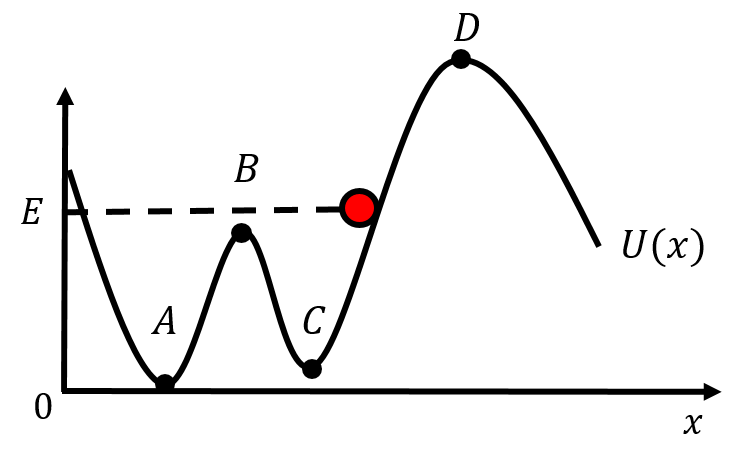
\includegraphics[width=0.6\linewidth]{files/potential-e092acd863f57ea581351938e0c3506c.png}
\caption[]{Arbitrary potential energy function and illustration of visualizing a marble rolling down the function by placing the marble on the potential energy function at a point where $U(x)=E$.}
\label{fig:potentialecons:potential}
\end{figure}

The motion of the marble will be bound between the two points where the potential energy function is equal to $E$. When the marble is placed as shown, it will roll towards the left, just as if it were a real marble on a track. Since the potential energy is increasing as a function of $x$ at the point where we placed the marble, the force is in the negative $x$ direction (remember, the force is the negative of the derivative of the potential energy function). With the given energy, the marble would never be able to make it to point $D$, as it does not have enough energy to ``climb up the hill''. It would roll down, through point $C$, up to point $B$, down to point $A$, and then turn around where $U(x)=E$ and return to where it started.

Locations $A$ and $C$ on the diagram are stable equilibria, because if a marble is placed in one of those locations and nudged slightly, it will come back to the equilibrium point (or oscillate about that point). Points $B$ and $D$ are ``unstable equilibria'', because if the marble is placed there and nudged, it will not immediately come back to those points. Note that if the marble were placed at point $D$ and nudged towards the right, the motion of the marble would be unbound on the right, and it would keep going in that direction.

Now, say an object's potential energy is described by the function in Figure~\ref{fig:potentialecons:potential}, and the object has total energy $E$. The object's motion along the $x$ axis will be exactly the same as the projection of the marble's motion on the $x$ axis.

\begin{framed}
\textbf{Checkpoint}\\
A force, $F(x)$, acts on an object. The potential energy function, $U(x)$, associated with the force is given by $U(x)=a(x -6)^2(x -1)(x -3)+20 {\rm J}$, where $a$ is a positive constant. $U(x)$ is plotted in Figure~\ref{fig:potentialecons:potentialcheckpoint}. Use the ``marble'' method to determine the direction of the force at $x=5$. Confirm your answer by finding the value of the force , $F(x)$, at $x=5$.

\begin{figure}[!htbp]
\centering
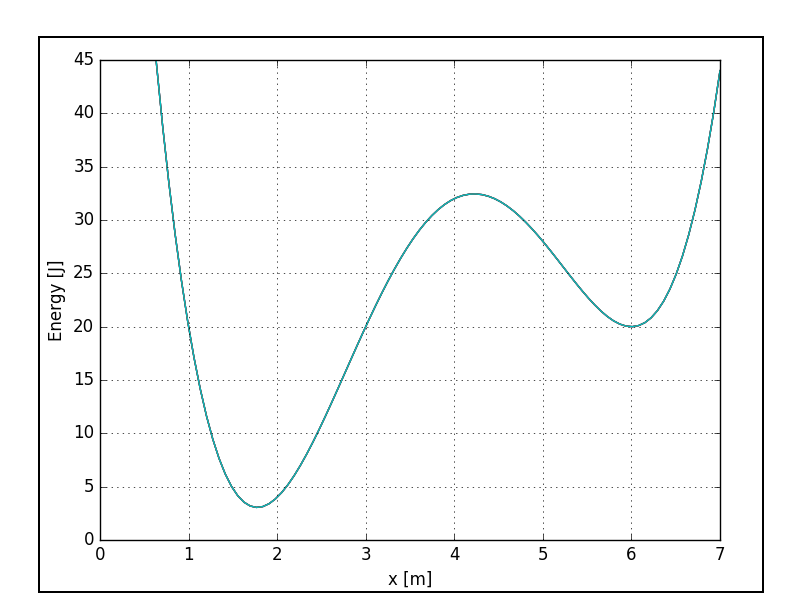
\includegraphics[width=0.5\linewidth]{files/potentialcheckpoint-611b04b42e2cece8657bac4b1784030f.png}
\caption[]{A potential energy function $U(x)$. The $x$-axis represents the $x$ position and the $y$-axis represents the energy.}
\label{fig:potentialecons:potentialcheckpoint}
\end{figure}

\begin{enumerate}
\item $F(x=5)= -10a$
\item $F(x=5)=10a$
\item $F(x=5)=20a$
\item $F(x=5)= -20a$
\end{enumerate}

\begin{framed}
\textbf{Answer}\\
\begin{enumerate}[resume]
\item
\end{enumerate}
\end{framed}
\end{framed}

\subsubsection{Advanced Topic: The Lagrangian formulation of classical physics}

So far, we have seen that, based on Newton's Laws, one can formulate a description of motion that is based solely on the concept of energy. A lot of research was done in the eighteenth century to reformulate a theory of mechanics that would be equivalent to Newton's Theory but whose starting point is the concept of energy instead of the concept of force. This ``modern'' approach to classical mechanics is primarily based on the research by Lagrange and Hamilton.

Although it is beyond the scope of this text to go into the details of this formulation, it is worth taking a quick look in order to get a better sense of how physicists seek to generalize theories. It is also worth noting that the Lagrangian formulation is the method by which theories are developed for quantum mechanics and modern physics.

The Lagrangian description of a ``system'' is based on a quantity, $L$, called the ``Lagrangian'', which is defined as:
\begin{equation}
\boxed{L = K - U}
\end{equation}
where $K$ is the kinetic energy of the system, and $U$ is its potential energy. A ``system'' can be a rather complex collection of objects, although we will illustrate how the Lagrangian formulation is implemented for a single object of mass $m$ moving in one dimension under the influence of gravity. Let $x$ be the direction of motion (which is vertical) such that the potential and kinetic energies of the object are given by:
\begin{equation}
U(x) &= mgx\\
K(v_x) &= \frac{1}{2}mv_x^2\\
\therefore L(x,v_x) &= \frac{1}{2}mv_x^2 - mgx
\end{equation}
where we chose the potential energy to be zero at $x=0$, and $v_x$ is the velocity of the object.

In the modern formulation of classical mechanics, the motion of the system will be such that the following integral is minimized:
\begin{equation}
S = \int Ldt
\end{equation}
where $L$ can depend on time explicitly or implicitly (through the fact that position and velocity, on which the Lagrangian depends, are themselves time-dependent). The requirement that the above integral be minimized is called the ``Principle of Least Action''\footnote{The integral, $S$, is called the ``action'' of the system.}, and is thought to be the fundamental principle that describes all of the laws of physics. The condition for the action to be minimized is given by the Euler-Lagrange equation:
\begin{equation}
\boxed{\frac{d}{dt}\left(\frac{\partial L}{\partial v_x}\right)-\frac{\partial L}{\partial x} = 0}
\end{equation}
Thus, in the Lagrangian formulation, one first writes down the Lagrangian for the system, and then uses the Euler-Lagrange equation to obtain the ``equations of motion'' for the system (i.e. equation that give the kinematic quantities, such as acceleration, for the system).

Given the Lagrangian that we found above for a particle moving in one dimension under the influence of gravity, we can determine each term in the Euler-Lagrange equation:
\begin{equation}
\frac{\partial L}{\partial v_x} &= \frac{\partial }{\partial v_x}\left(\frac{1}{2}mv_x^2 - mgx \right)=mv_x\\
\therefore\frac{d}{dt}\left(\frac{\partial L}{\partial v_x}\right) &= \frac{d}{dt} (mv_x) = ma_x\\
\frac{\partial L}{\partial x}&= \frac{\partial }{\partial x}\left(\frac{1}{2}mv_x^2 - mgx\right) = -mg\\
\end{equation}
Putting these into the Euler-Lagrange equation:
\begin{equation}
\frac{d}{dt}\left(\frac{\partial L}{\partial v_x}\right)-\frac{\partial L}{\partial x} &= 0\\
(ma_x) - (-mg) &=0\\
ma_x&=-mg\\
\therefore a_x &= -g
\end{equation}
which is exactly equivalent to using Newton's Second Law (the second last step is equivalent to $F=ma$). In the Lagrangian formulation, we do not need the concept of force. Instead, we describe possible ``interactions'' by a potential energy function. That is why you may sometimes hear of physicists talking about the ``Weak interaction'' instead of the ``Weak force'' when they are talking about one of the four fundamental interactions (forces) of Nature. This is because, in the modern formulation of physics, one does not use the concept of force, and instead thinks of potential energy functions to model what we would call a force in the Newtonian approach.

Emmy Noether, a mathematician in the early twentieth century, proved a theorem that makes the Lagrangian formulation particularly aesthetic.
Noether's theorem states that for any symmetry in the Lagrangian, there exists a quantity that is conserved. For example, if the Lagrangian does not depend explicitly on time, then a quantity, which we call energy, is conserved\footnote{If the Lagrangian does not depend on time, then we can shift the system in time and the equations of motion would be unaffected. We say that the Lagrangian is symmetric, or unaffected, by changes in time.}.

The Lagrangian that we had above for a particle moving under the influence of gravity did not depend on time explicitly, and thus energy is conserved (gravitational potential energy is converted into kinetic energy and there are no non-conservative forces). If the Lagrangian did not depend on position, then a quantity that we call ``momentum''\footnote{See Section~\ref{chap:momentumandcm}.} would be conserved. In this case, momentum in the $x$ direction was not conserved because the Lagrangian depended on $x$ through the potential energy.

\begin{framed}
\textbf{Olivia's Thoughts}\\
We saw in this chapter that describing systems in terms of energy is often easier than describing them in terms of forces. The Lagrangian gives us a way to get the same information we would get from Newton's laws (like the acceleration, etc.), but using energy as a starting point. The Lagrangian method is really useful when we are looking at motion in multiple dimensions, or when we are describing complicated systems. Using the Lagrangian is actually really simple, and just like with forces, you can pretty much approach every problem the same way. Here are the basic steps to follow:

\begin{enumerate}
\item Find two expressions for your system: one for the potential energy ($U$) and one for the kinetic energy ($K$). This often ends up being the hardest step.
\item Write down the Lagrangian, $L=K -U$, using the expressions you just found.
\item Pick a coordinate. (In one dimension, this is trivial, but it will be important once you start working in multiple dimensions). The Euler-Lagrange equation was given to you as:
\end{enumerate}
\begin{equation}
\frac{d}{dt}\left(\frac{\partial L}{\partial v_x}\right)-\frac{\partial L}{\partial x} = 0
\end{equation}
because we are working in one dimension. You can actually pick whichever coordinate you are interested in. For example, if you were interested in the motion of your object in the $y$ direction, you would pick $y$ as your coordinate and write:
\begin{equation}
\frac{d}{dt}\left(\frac{\partial L}{\partial v_y}\right)-\frac{\partial L}{\partial y} = 0
\end{equation}
\begin{enumerate}[resume]
\item Now you just have to do what the equation above tells you to do, which is to start with your Lagrangian (your $L=K -U$ equation) and take a bunch of derivatives. If you try to just plug $L$ into the Euler-Lagrange equation and do all the derivatives at once, it can get confusing. I recommend finding the components separately. I like to start by taking the partial derivative with respect to velocity, $\frac{\partial L}{\partial v_y}$, then taking its derivative with respect to time. Next, I find $\frac{\partial L}{\partial y}$ and then put it all together.
\item That's it! When you've taken the derivatives (and simplified a bit), you'll have an ``equation of motion'' that gives you information about the motion of the object. You can then use this equation however you want!
\end{enumerate}
\end{framed}

\subsubsection{Summary}

A force is conservative if the work done by that force on a closed path is zero:
\begin{equation}
\oint \vec F(\vec r) \cdot d\vec l = 0
\end{equation}
Equivalently, the force is conservative if the work done by the force on an object moving from position $A$ to position $B$ does not depend on the particular path between the two points. The conditions for a force to be conservative are given by:
\begin{equation}
\frac{\partial F_z}{\partial y}-\frac{\partial F_y}{\partial z} &= 0 \nonumber\\
\frac{\partial F_x}{\partial z}-\frac{\partial F_z}{\partial x} &= 0\nonumber\\
\frac{\partial F_y}{\partial x}-\frac{\partial F_x}{\partial y} &= 0
\end{equation}
In particular, a force that is constant in magnitude and direction will be conservative. A force that depends on quantities other than position (e.g. speed, time) will not be conservative. The force exerted by gravity and the force exerted by a spring are conservative.

For any conservative force, $\vec F(\vec r)$, we can define a potential energy function, $U(\vec r)$, that can be used to calculate the work done by the force along any path between position $A$ and position $B$:
\begin{equation}
-W = - \int_A^B \vec F(\vec r) \cdot d\vec l = U(\vec r_B) - U(\vec r_A) = \Delta U
\end{equation}
where the change in potential energy function in going from $A$ to $B$ is equal to the negative of the work done in going from point $A$ to point $B$. We can determine the function $U(\vec r)$ by calculating the work integral over an ``easy'' path (e.g. a straight line that is co-linear with the direction of the force).

It is important to note that an arbitrary constant can be added to the potential energy function, because only differences in potential energy are meaningful. In other words, we are free to choose the location in space where the potential energy function is defined to be zero.

We can break up the net work done on an object as the sum of the work done by conservative ($W^C$) and non-conservative forces ($W^{NC}$):
\begin{equation}
W^{net}&=W^{NC}+W^{C}=W^{NC}-\Delta U
\end{equation}
where $\Delta U$ is the difference in the total potential energy of the object (the sum of the potential energies for each conservative force acting on the object).

The Work-Energy Theorem states that the net work done on an object in going from position $A$ to position $B$ is equal to the object's change in kinetic energy:
\begin{equation}
W^{net}&=\frac{1}{2}mv_B^2-\frac{1}{2}mv_A^2=\Delta K
\end{equation}
We can thus write that the total work done by non conservative forces is equal to the change in potential and kinetic energies:
\begin{equation}
W^{NC}=\Delta K+\Delta U
\end{equation}
In particular, if no non-conservative forces do work on an object, then the change in total potential energy is equal to the negative of the change in kinetic energy of the object:
\begin{equation}
-\Delta U=\Delta K
\end{equation}
We can introduce the mechanical energy, $E$, of an object as:
\begin{equation}
E = U+K
\end{equation}
The net work done by non-conservative forces is then equal to the change in the object's mechanical energy:
\begin{equation}
W^{NC}=\Delta E
\end{equation}
In particular, if no net work is done on the object by non-conservative forces, then the mechanical energy of the object does not change ($\Delta E=0$). In this case, we say that the mechanical energy of the object is conserved.

The Lagrangian description of classical mechanics is based on the Lagrangian, $L$:
\begin{equation}
L = K - U
\end{equation}
which is the difference between the kinetic energy, $K$, and the potential energy, $U$, of the object. The equations of motion are given by the Principle of Least Action, which leads to the Euler-Lagrange equation (written here for the case of a particle moving in one dimension):
\begin{equation}
\frac{d}{dt}\left(\frac{\partial L}{\partial v_x}\right)-\frac{\partial L}{\partial x} = 0
\end{equation}

\begin{framed}
\textbf{Important Equations}\\
\textbf{Conditions for a force to be conservative:}
\begin{equation}
\oint \vec F(\vec r) \cdot d\vec l = 0
\end{equation}
\begin{equation}
\frac{\partial F_z}{\partial y}-\frac{\partial F_y}{\partial z} &= 0 \nonumber\\
\frac{\partial F_x}{\partial z}-\frac{\partial F_z}{\partial x} &= 0\nonumber\\
\frac{\partial F_y}{\partial x}-\frac{\partial F_x}{\partial y} &= 0
\end{equation}
\textbf{Potential energy for a conservative force:}
\begin{equation}
\Delta U&=-W\\
U(\vec r_B) - U(\vec r_A)&= - \int_A^B \vec F(\vec r) \cdot d\vec l
\end{equation}

\textbf{Work-energy theorem:}
\begin{equation}
W^{net}&=\frac{1}{2}mv_B^2-\frac{1}{2}mv_A^2=\Delta K
\end{equation}
\textbf{Work:}
\begin{equation}
W^{net}&=W^{NC}+W^{C}=W^{NC}-\Delta U\\
W^{NC}&=\Delta K+\Delta U
\end{equation}
\textbf{Energy:}
\begin{equation}
E&=U+K\\
W^{NC}&=\Delta E
\end{equation}
\textbf{Lagrange:}
\begin{equation}
L = K - U\\
\frac{d}{dt}\left(\frac{\partial L}{\partial v_x}\right)-\frac{\partial L}{\partial x} = 0
\end{equation}
\end{framed}

\begin{framed}
\textbf{Important Definitions}\\
\begin{itemize}
\item \textbf{Conservative force:} A force that does no net work when exerted over a closed path.
\item \textbf{Potential energy:} A form of energy that an object has by virtue of its position in space. The potential energy is associated with a conservative force, which is exerted in the direction that lowers the potential energy of the object. SI units: ${\rm \left[{J}\right]}$. Common variable(s): $U$.
\end{itemize}
\end{framed}

\subsubsection{Thinking about the material}

\begin{framed}
\textbf{Reflect and research}\\
\begin{itemize}
\item When did Lagrange publish his theory of classical mechanics, and what was the name of the publication?
\item What is D'Alembert's contribution to the field of classical mechanics?
\item Who first proposed the Principle of Least Action, and when?
\item What is an example of a situation not already covered that you can describe where mechanical energy is conserved?
\item Under what symmetry is angular momentum conserved?
\item Think of three renewable energy sources and describe how they use conservation of energy to produce electricity.
\item What is a Rube Goldberg machine? Look up some videos of Rube Goldberg machines, and find the coolest one!
\end{itemize}
\end{framed}

\begin{framed}
\textbf{To try at home}\\
\begin{itemize}
\item Design a small catapult or slingshot that you can build using materials found at home. Describe how these machines work using conservation of energy.
\end{itemize}
\end{framed}

\begin{framed}
\textbf{To try in the lab}\\
\begin{itemize}
\item Propose an experiment to test that energy is conserved in a system where only gravity acts.
\item Simulate the launch of a space probe out of the solar system using a gravity assist.
\item Model and investigate the craters that are created when objects are dropped into a bed of sand.
\end{itemize}
\end{framed}

\subsubsection{Sample problems and solutions}

\paragraph{Problems}

\begin{framed}
\textbf{Problem 8.1}\\
\begin{figure}[!htbp]
\centering
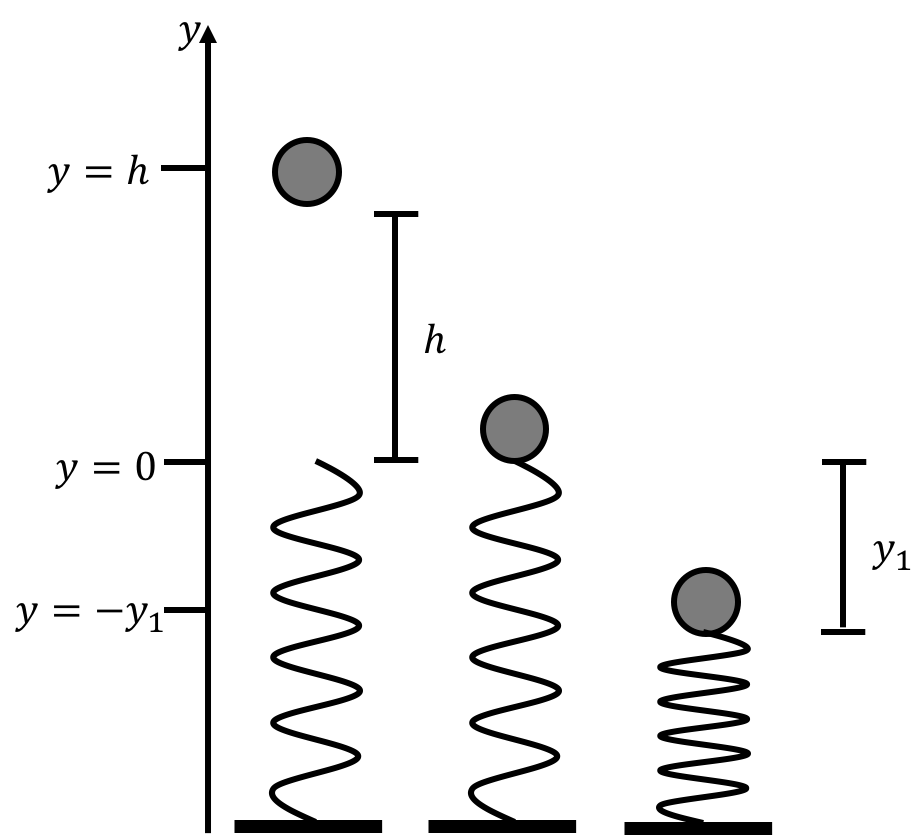
\includegraphics[width=0.4\linewidth]{files/massdropspring-f73fe0e55835506b4148fcc4430499ee.png}
\caption[]{A ball is dropped from rest onto a vertical spring.}
\label{fig:potentialecons:ballspring}
\end{figure}
\end{framed}

\begin{framed}
\textbf{Problem 8.2}\\
A simple pendulum consists of a mass $m$ connected to a string of length $L$. The pendulum is released from an angle $\theta_0$ from the vertical. Use conservation of energy to find an expression for the velocity of the mass as a function of the angle.

\begin{figure}[!htbp]
\centering
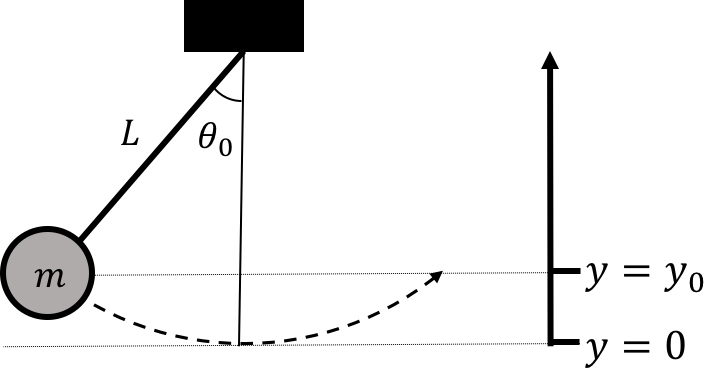
\includegraphics[width=0.4\linewidth]{files/pendulumvelocity-130b363d2f37b84b8531059415885194.png}
\caption[]{A pendulum is released from rest an angle $\theta_0$ from the vertical.}
\label{fig:potentialecons:pendulumvel}
\end{figure}
\end{framed}

\begin{framed}
\textbf{Problem 8.3}\\
A block of mass $m$ sits on a frictionless horizontal surface. It is attached to a wall by a spring with a spring constant $k$. The mass is pushed so as to compress the spring and then it is released (Figure~\ref{fig:potentialecons:springmassoscillate}). Use the Lagrangian formalism to find an equation of motion for the mass/spring system (i.e. use the Lagrangian to determine the acceleration of the mass).

\begin{figure}[!htbp]
\centering
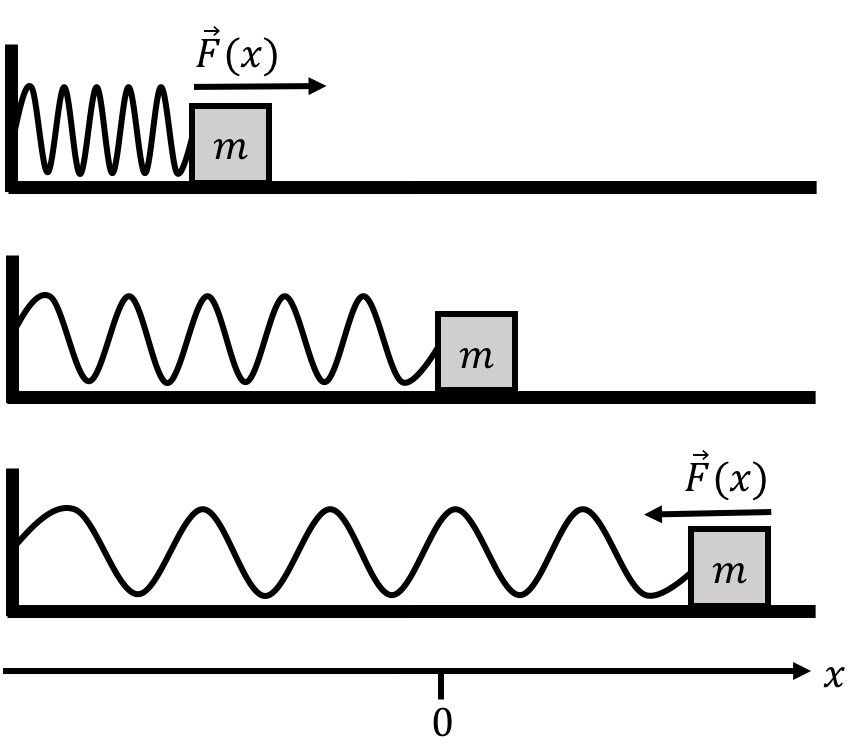
\includegraphics[width=0.4\linewidth]{files/massoscillating-022f0299125fb833304e7dba4fbb0cfe.png}
\caption[]{A mass attached to a spring oscillates about the rest position of the spring.}
\label{fig:potentialecons:springmassoscillate}
\end{figure}
\end{framed}

\paragraph{Solutions}

\begin{framed}
\textbf{Solution 8.1}\\
The two forces acting on the ball are gravity and the spring force. Both are conservative, so we can use conservation of mechanical energy. We will find the energy of the ball when it is at a height $h$ above the spring, and the energy of the ball when the spring is fully compressed. Then, we will use conservation of mechanical energy to determine the compression of the spring.

Remember that the total mechanical energy is the sum of the total potential energy and the kinetic energy, $E=U+K$. Let's call the initial position of the ball $A$ and the final position of the ball $B$. You will notice that we set up our coordinate system so that $y$ is positive upwards, with $y=0$ at the point where the ball comes into contact with the spring. We choose to define both the gravitational potential energy and spring potential energy so that they are zero at $y=0$.

Since the ball starts from rest, its kinetic energy is zero at position $A$. At this point, the ball is not touching the spring, so the potential energy from the spring force is zero. The mechanical energy of the ball at position $A$ is simply equal to its gravitational potential energy:
\begin{equation}
E_A&=U_A+K_A\\
E_A&=mgh
\end{equation}
At position $B$, the ball is again at rest, so the kinetic energy of the ball is zero. Now that the ball is in contact with the spring, it will experience a force from the spring that can be modelled with a potential energy $U(y)=\frac{1}{2}ky_1^2$, where $y_1$ is the distance between the rest position of the spring and its compressed length. At point $B$ ($y= -y_1$), the ball will have both spring and gravitational potential energy, so its mechanical energy at position $B$ is given by:
\begin{equation}
E_B&=U_B+K_B=U_B\\
U_B&=mg(-y_1)+\frac{1}{2}ky_1^2\\
E_B&=-mgy_1+\frac{1}{2}ky_1^2
\end{equation}
Since mechanical energy is conserved in this system (no non-conservative forces are doing work), we can now set $E_A=E_B$ and solve for $y_1$:
\begin{equation}
E_A&=E_B\\
mgh&=-mgy_1+\frac{1}{2}ky_1^2\\
0&=\frac{1}{2}ky_1^2-mgy_1-mgh\\
\end{equation}
where in the last line we rewrote the expression as a quadratic equation. We can solve for $y_1$ with the quadratic formula:
\begin{equation}
y_1=\frac{mg\pm\sqrt{(mg)^2-4(1/2k)(-mgh)}}{k}\\
y_1=\frac{mg\pm\sqrt{mg(mg+2kh)}}{k}
\end{equation}
We now have an expression for the amount the spring is compressed, $y_1$, in terms of our known values.
\end{framed}

\begin{framed}
\textbf{Solution 8.2}\\
We are going to find a general expression for the energy of the system, and then use this expression to find the velocity at any point. There are two forces acting on the mass:

\begin{enumerate}
\item The force of tension (from the string). This force is perpendicular to the direction of motion at any point, so it does no work on the mass.
\item The force of gravity, which has a potential energy function given by $U(y)=mgy$. We choose the gravitational potential energy to be zero when the pendulum hangs vertically (when $\theta=0$ and $y=0$).
\end{enumerate}

The mechanical energy of the mass is conserved, and at any point is given by the sum of its kinetic and its gravitational potential energies:
\begin{equation}
E=mgy+\frac{1}{2}mv^2
\end{equation}
We want to find the velocity as a function of $\theta$, so we need to write $y$ in terms of $\theta$. As you may recall from Figure~\ref{fig:workenergy:swingprob}, we saw that from the geometry of the problem, we can express the height of the mass as $y=L -L\cos\theta$, or $L(1 -\cos\theta)$, where $y$ is the height as measured from the bottom point of the motion. You can refer to Figure~\ref{fig:workenergy:swingprobgeometry} to refresh your memory. The energy at any point is then:
\begin{equation}
E=mgL(1-\cos\theta)+\frac{1}{2}mv^2
\end{equation}
Conservation of energy tells us that the total energy at any point must be the same as the initial energy. So, we can use our initial conditions to find the total energy of the system. The mass starts from rest (initial kinetic energy is zero) an angle $\theta_0$ above the vertical:
\begin{equation}
E&=mgL(1-\cos\theta)+\frac{1}{2}mv^2\\
E_{initial}&=mgL(1-\cos\theta_0)
\end{equation}
Now that we have found the total energy of the system, we can write our general expression for the energy of the system at any point:
\begin{equation}
E&=mgL(1-\cos\theta)+\frac{1}{2}mv^2\\
mgL(1-\cos\theta_0)&=mgL(1-\cos\theta)+\frac{1}{2}mv^2
\end{equation}
All that's left to do is simplify the expression and rearrange for $v$:
\begin{equation}
mgL(1-\cos\theta_0)&=mgL(1-\cos\theta)+\frac{1}{2}mv^2\\
gL(1-\cos\theta_0)-gL(1-\cos\theta)&=\frac{1}{2}v^2\\
gL-gL\cos\theta_0-gL+gL\cos\theta&=\frac{1}{2}v^2\\
gL(\cos\theta-\cos\theta_0)&=\frac{1}{2}v^2\\
\therefore v&=\sqrt{2gl(\cos\theta-\cos\theta_0)}
\end{equation}
\textbf{Discussion:} We can see from this expression that the speed will be maximized when $\cos\theta$ is maximized, which will occur when $\theta=0$ (when the pendulum is vertical). This is as we expected. We can also see that we will get an imaginary number if the magnitude of $\theta$ is greater than $\theta_0$, showing that the motion is constrained between $-\theta_0$ and $\theta_0$. Finally, we showed that the velocity of the pendulum does not depend on the mass!
\end{framed}

\begin{framed}
\textbf{Solution 8.3}\\
We are going to find an equation of motion of the system using the Lagrangian method. We choose to use a one dimension coordinate system, with the $x$ axis defined to be co-linear with the spring, positive in the direction where the spring is extended, and set the origin to be located at the rest position of the spring. The kinetic energy and potential energy of the mass are given by
\begin{equation}
K&=\frac{1}{2}mv_x^2\\
U&=\frac{1}{2}kx^2
\end{equation}
since the only force exerted on the mass that can do work is the force from the spring. We have chosen the potential energy to be zero at $x=0$. The Lagrangian for this system is:
\begin{equation}
L&=K-U\\
L&=\frac{1}{2}mv_x^2-\frac{1}{2}kx^2
\end{equation}
The Euler-Lagrange equation in one dimension is:
\begin{equation}
\frac{d}{dt}\left(\frac{\partial L}{\partial v_x}\right)-\frac{\partial L}{\partial x} = 0
\end{equation}
We can calculate the terms of the Euler-Lagrange equation:
\begin{equation}
\frac{\partial L}{\partial v_x}&=\frac{\partial }{\partial v_x}\left(\frac{1}{2}mv_x^2-\frac{1}{2}kx^2\right)\\
&=mv_x\\
\therefore \frac{d}{dt}\left(\frac{\partial L}{\partial v_x}\right)&=\frac{d}{dt}(mv_x)\\
&=ma_x\\
\textrm{and}\qquad \frac{\partial L}{\partial x}&=\left(\frac{1}{2}mv_x^2-\frac{1}{2}kx^2\right)\\
&=-kx
\end{equation}
and then put them together to get:
\begin{equation}
\frac{d}{dt}\left(\frac{\partial L}{\partial v_x}\right)-\frac{\partial L}{\partial x} &= 0\\
\therefore ma_x&=-kx\\
\end{equation}
We can see that this equation of motion is equivalent to Newton's Second Law.
\end{framed}